\section{Reducing the MPI grid setup and initial load balancing overhead}


\chapterDescription
  {
    Around 30 minutes.
  }
  {
    A working MPI code.
  }


In this section, we assume that you've a reasonable load balancing and that you
were able to postprocess your performance analysis outputs. We discuss 


\paragraph{The smell}

\begin{center}
  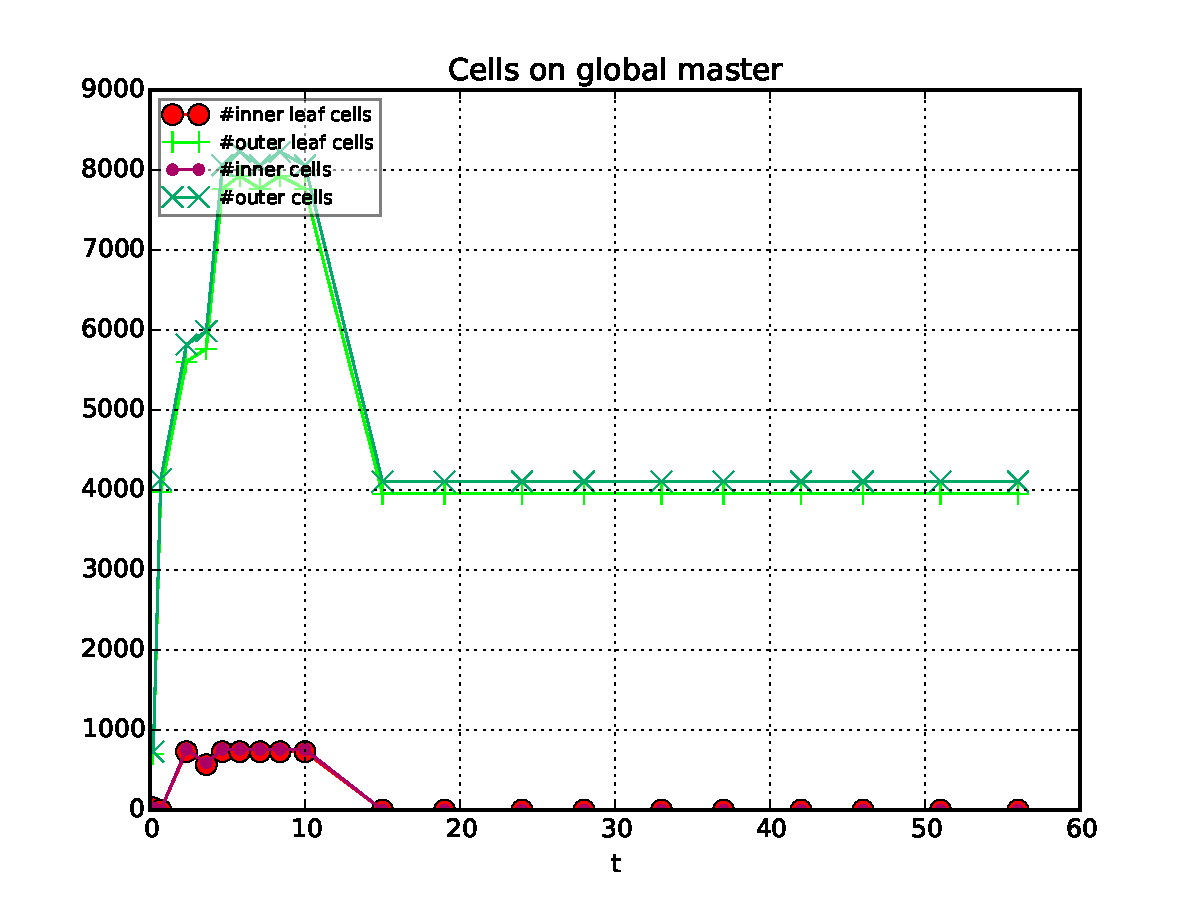
\includegraphics[width=0.5\textwidth]{41_mpi-setup/performance-analysis-output.pdf}
\end{center}



If you identify ranks whose local load decreases incrementally, these are ranks
that step by step fork more of their work to other ranks. 
In principle, this is fine and a result of load balancing. 
For reasonably static setups, it however is irritating: 
why is there such a long setup phase where obviously solely data is
redistributed?

The reason can be found in the semantics of \texttt{createVertex} and
\texttt{touchVertexFirstTime}.
Both operations try to refine the grid around the respective vertex immediately. 
Only if circumstances such as a parallel partitioning running through this
vertex---the refinement instruction then first has be distributed to all ranks
holding a copy of this vertex---do not allow Peano to realise the refinement
immediately, the refinement is postponed to the next iteration.
In many parallel codes, all the refinement calls pass through immediately on
rank 0 before it can spawn any rank.
This leads to the situation that the whole grid is in one sweep built up on the
global master and afterwards successively distributed among the ranks.


Such a behaviour is problematic: the global rank might run out of memory, lots
of data is transferred, and the sweeps over the whole grid on rank 0 are
typically pretty expensive. 
A distributed grid setup is advantageous.

\paragraph{The solution}

To facilitate this, it makes sense to switch from an aggressive
refinement into an iterative grid refinement strategy (one refinement level per
step, e.g.) to allow the rank to deploy work throughout the grid construction
and thus build up the grid in parallel and avoid the transfer of whole grid
blocks due to rebalancing.
Simply move your \texttt{refine()} call from the creational or touch first
events into \texttt{touchVertexLastTime()}:
As a consequence, setting up a (rather regular) grid of depth k requires at least k iterations. 


To find out when a grid has been constructed and balanced completely, the
repository provides an operation. Instead of writing something along the lines

\begin{code}
  repository.switchToSetup();
  repository.iterate();
\end{code}

\noindent
you have to write
\begin{code}
  repository.switchToSetupExperiment();
  do {
    repository.iterate();
  } while ( !repository.getState().isGridBalanced() );
\end{code}



\paragraph{Related pitfalls \& ideas}

As always, the devil is in the details:
\begin{itemize}
  \item  For many load balancing algorithms, it does make sense to create an
  initial grid of depth $\hat k <k$ on your rank 0 before you do any load
  balancing. This allows the load balancing metric to get a first idea about
  what the grid will look like and then to switch on load
  balancing. This can be done with
  \begin{code}
  peano::parallel::loadbalancing::Oracle::getInstance().activateLoadBalancing(false);
  // set up grid up to a certain level
  peano::parallel::loadbalancing::Oracle::getInstance().activateLoadBalancing(true);
  \end{code}
  \item Once all ranks have obtained `their' partition, it does not make sense
  to continue to build up at most one grid level per sweep. In this case, you
  have to reliase an inverse pattern compared to the pattern sketched in the
  first bullet point. Such a situation is easy to spot: it typically
  materialises in a slow increase of total/global vertices while the fork
  statistics show that no forks happen anymore. Compare the two plots below:
  \begin{center}
    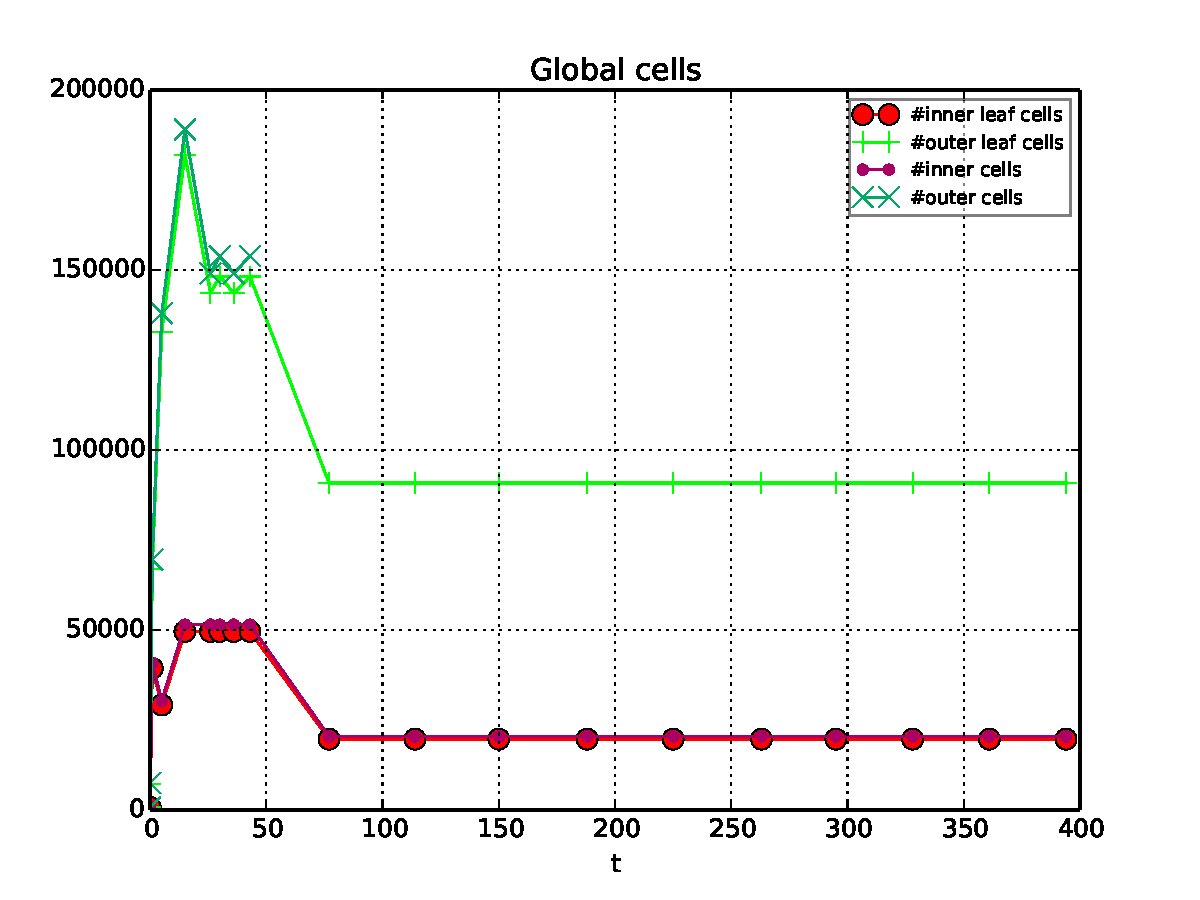
\includegraphics[width=0.4\textwidth]{41_mpi-setup/grid-construction.pdf}
    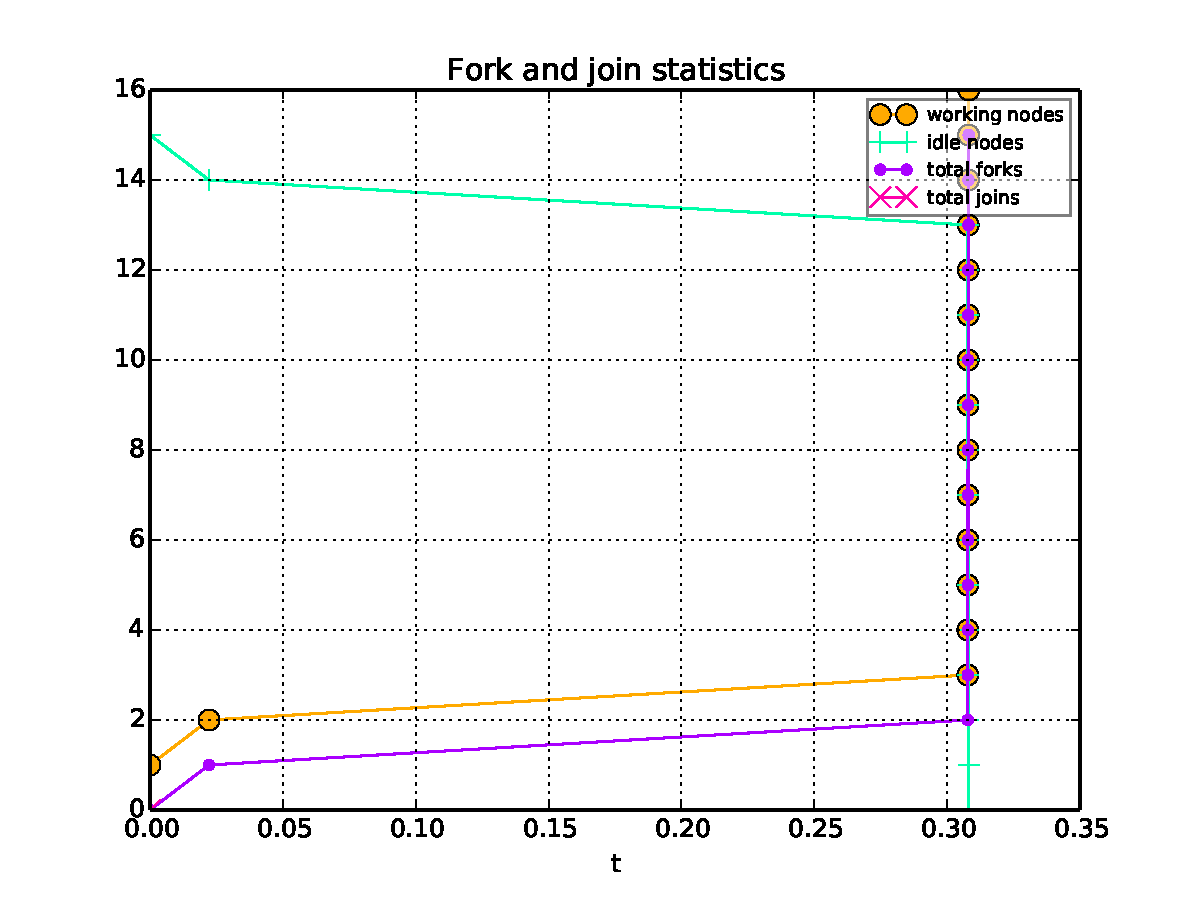
\includegraphics[width=0.4\textwidth]{41_mpi-setup/fork-behaviour.pdf}
    \\
    {
    \footnotesize
    }
  The grid construction requires about 80s while the last forks are tracked
  at t=0.3s. Starting from t=0.3s, one could build up the grid one sweep.
  \end{center}
  \begin{remark}
    Peano parallel code offers an operation \texttt{enforceRefine()} on
    the vertices that you can use to tackle this problem. Use with care and 
    read through the documentation in code.
  \end{remark}
  \item Everytime you rebalance your grid, Peano disables dynamic load balancing
  for a couple of iterations (three or four). Throughout these iterations, it
  can recover all adjacency information if the grid itself changes as well.
  Consequently, it does make sense to add a couple of adapter runs after each
  grid modification that to not change the grid structure: When you know that
  you have an adapter that changes the grid, apply afterwards an adapter that
  does not change the grid for a couple of times. This way, you ensure that no
  mpi rank runs out of memory. The grid generation does not overtake the rebalancing.
  \item If you are using the heap data structure, it furthermore makes sense to split up
the initialisation into a grid setup and a data struture initialisation.
You balance and distribute the grid setup following the recommendations above
and then in one additional sweep initialise the heap.
You initialise the heap as late as possible and thus avoid unneccesary
administrative overhead.
\end{itemize}


\paragraph{Pattern for static grid setup}

Most codes at least start form a static grid partitioning and globally know
what the initial grid looks like.
It then has proven of value to do the following:

\begin{enumerate}
  \item Determine a certain grid level that should be used to do an initial load
  balancing. If you have a regular grid, this might be the coarsest grid level
  that could be deployed among all involved ranks:
  \begin{code}
_coarsestRegularLevelUsedForDD = 0;
int ranksUsedSoFar             = 0;
int increment                  = 1;
while (ranksUsedSoFar < tarch::parallel::Node::getInstance().getNumberOfNodes()) {
  ranksUsedSoFar += increment;
  increment      *= THREE_POWER_D;
  _coarsestRegularLevelUsedForDD ++;
}
  \end{code}
  Typically, I determine this level in \texttt{beginIteration()} of the mapping
  that constructs the initial grid. It is thus determined in parallel on all
  ranks as soon as a rank joins the game.
  \item I make the grid setup refine the grid in \texttt{touchVertexLastTime},
  i.e.~the grid is created with one level per sweep. As this part of the code
  runs in parallel, we run over the grid $k'$ times, add one level per sweep (so
  $k'$ becomes the depth of the tree), and at the same time distribute the grid
  among the ranks. We successively flood the MPI nodes. However, we continue to
  add new levels if and only if we do not exceed the initial grid depth
  determined in step 1:
  \begin{code}
...::touchVertexLastTime(...) {
  if (
    shallRefine(fineGridVertex,fineGridH)
    &&
    coarseGridVerticesEnumerator.getLevel() < _coarsestRegularLevelUsedForDD
  ) {
    fineGridVertex.refine();
  }
  ...
}  
  \end{code}
  \item I make all the ranks switch off dynamic load balancing the first time
  the global master runs a step on all ranks out there:
  \begin{code}
void picard::runners::Runner::runGlobalStep() {
  // assertion( !peano::parallel::loadbalancing::Oracle::getInstance().
  // isLoadBalancingActivated() );

  peano::parallel::loadbalancing::Oracle::getInstance().activateLoadBalancing(false);
}
  \end{code}
  For this, I remove the assertion original put in by PDT. I know what I'm
  doing, as \ldots
  \item I run through the grid until it becomes stationary, i.e.~does not change
  anymore and is properly distributed. Due to the variable
  \texttt{\_coarsestRegularLevelUsedForDD} this will require a couple of sweeps
  but will not set up the whole grid. Next, I switch off load balancing
  globally. Finally, I rerun the grid construction twice. The runner then
  resembles
  \begin{code}
repository.switchToCreateGrid();
do {
  repository.iterate();
} while ( !repository.getState().isGridBalanced() );

repository.runGlobalStep();
runGlobalStep();

repository.iterate();
repository.iterate();
  \end{code}
  \item So far, the last two iterates do not change the grid anymore and they
  notably do not build up the whole grid if the grid is truncated by
  \texttt{\_coarsestRegularLevelUsedForDD}. I finally return to the mapping's
  touch vertex last time event and continue to refine if the load balancing is
  switched off. This refinement will kick in the in first of the two additional
  \texttt{iterate} commands.
  \begin{code}
...::touchLastTime(...) {
  if (
    shallRefine(fineGridVertex,fineGridH)
    &&
    !peano::parallel::loadbalancing::Oracle::getInstance().isLoadBalancingActivated()
  ) {
    fineGridVertex.refine();
  }
}
  \end{code}
  \item This new fragment will make the last \texttt{iterate} introduce one
  additional level that is finer than \texttt{\_coarsestRegularLevelUsedForDD}. 
  When it invokes the corresponding creational routines, we now use
  \texttt{enforceRefine} to build up the remaining grid parts in one sweep. 
  \begin{code}
...::createInnerVertex(...) {
  if ( 
    shallRefine(fineGridVertex,fineGridH) 
    &&
    !peano::parallel::loadbalancing::Oracle::getInstance().isLoadBalancingActivated()
  ) {
    fineGridVertex.enforceRefine();
  }

}
\end{code}
  Exactly the same has to be done within \texttt{createBoundaryVertex}.
\end{enumerate}



